\documentclass[12pt]{report}
\usepackage[T2A]{fontenc} % Use 8-bit encoding that has 256 glyphs

\usepackage[utf8]{inputenc} % Required for including letters with accents

\usepackage[english,russian]{babel}
\usepackage{cmap}

\usepackage{indentfirst}
\setlength{\parindent}{0pt}

\usepackage{graphicx} % Required for including images
\graphicspath{{Figures/}} % Set the default folder for images

\usepackage{enumitem} % Required for manipulating the whitespace between and within lists

\usepackage{lipsum} % Used for inserting dummy 'Lorem ipsum' text into the template

\usepackage{subfig} % Required for creating figures with multiple parts (subfigures)

\usepackage{varioref} % More descriptive referencing

\usepackage{assoccnt}

\usepackage[
    type={CC},
    modifier={by-nc-sa},
    version={4.0},
]{doclicense}

\usepackage{xpatch}

\usepackage{amsmath,amssymb,amsthm,amsfonts} % For including math equations, theorems, symbols, etc

\usepackage{multicol}
\usepackage{graphicx}
\graphicspath{ {./images/} }

\theoremstyle{plain} % жирный заголовок, наклонный текст
\newtheorem{thm}{Теорема}
\newtheorem{lem}{Лемма}
\newtheorem{utv}[thm]{Утверждение} %счетчик утверждений иcпользует счетчик теорем - [thm] после объявления имени
\newtheorem{sle}{Следствие}[thm] %счетчик следствий подчинен счетчику теорем - [thm] в конце
\newtheorem*{sle*}{Следствие} %звездочка после newtheorem убирает нумерацию
\newtheorem*{remark*}{Замечение}

\theoremstyle{definition}
\newtheorem{task}{Задача}
\newtheorem*{solution}{Решение}
%----------------------------------------------------------------------------------------
%	HYPERLINKS
%---------------------------------------------------------------------------------------
\usepackage{hyperref}

\hypersetup{
    colorlinks=true,
    linkcolor=blue,
    filecolor=magenta,      
    urlcolor=cyan,
    pdftitle={Overleaf Example},
    pdfpagemode=FullScreen,
    }

\setcounter{section}{1}

\title{
    Конспект по дискретной математике \\ 
    \large На основе лекций Рабиновича А.С
}    

\author{
    Рустамова Дарина
}
\date{\the\year}


\begin{document}
\maketitle
\tableofcontents

\newcommand\shortlorem{}

\newpage
% \doclicenseThis

\chapter{Теория множеств}
\section{Основные понятия}

\textbf{Множество} - это совокупность каких-либо объектов. 
Множества бывают конечными, бесконечными пустыми, счестными и бесчетными.

Мощность множества: $|A|$

Если между двумя множествами $A$ и $B$ можно установить взаимно-однозначное соответствие,
тогда множества называются \textbf{равномощными}.
\begin{equation}
    |A| = |B|
\end{equation}

\textbf{Теорема Кантора}. Множество подмножеств любого множества, имеет мощность больше,
чем само множество.

Обычно в множество подмножеств входит пустое множество и само множество.

Чтобы проверить теорему Кантора, рассмотрим конечное множество и рассмотрим множество
подмножеств конечного множества из n элементов. Например, рассмотрим множество из 2-х
элементов 
\begin{equation*}
    A = \{1, 2\} 
\end{equation*}

Множество подмножеств равно
\begin{equation*}
    A_2 = \{\emptyset, \{1\}, \{2\}, \{1, 2\}\}
\end{equation*}

Рассмотрим из множество 3-х элементов
\begin{equation*}
    B = \{1, 2, 3\} 
\end{equation*}

Множество подмножеств равно
\begin{equation*}
    B_3 = \{\emptyset, \{1\}, \{2\}, \{3\}, \{1, 2\}, \{1, 3\}, \{2, 3\}, \{1, 2, 3\}\}
\end{equation*}

Напрашивается закономерность, что
\begin{equation}
    |A_n| = 2^{|A|}
\end{equation}
где $|A_n|$ - мощность множества подможеств множества из n элементов

Выведем так же несколько формул для мощность множества подмножеств:
\begin{gather}
    |A_n| = |A_{n-1}| + |A_{n-1}| = 2|A_{n-1}|\\
    |A_n| = 2|A_{n-1}| = 2^{2}|A_{n-1}| = ... = 2^{n}|A_0| = 2^{n}
\end{gather}

Поставим вопрос: сколько будет подмножеств из n элементов содержащих k элементов? Отвечаю.
$C^{k}_n$ - число подмножеств из k элементов.

Стоит заметить, что
\begin{equation}
    \sum_{k=0}^{n} C^{k}_n = 2^{n}
\end{equation}

\section{Операции над множествами}

Рассмотрим основные операции над множествами.

\textbf{Объединение} 
\begin{equation}
    A \cup B = \{x: x \in A \cup x \in B\}
\end{equation}

\textbf{Пересечение} 
\begin{equation}
    A \cap B = \{x: x \in A \cap x \in B\}
\end{equation}

\textbf{Дополнение} 
\begin{equation}
    \overline A = \{x: x \notin A\}
\end{equation}

\textbf{Вычитание} 
\begin{equation}
    A \backslash B = \{x: x \in A \cap x \notin B\} = A \cap \overline B
\end{equation}

\textbf{Сумма} 
\begin{equation}
    A \oplus B = (A \backslash B) \cup (B \backslash A) = (A \cap \overline B) \cup (B \cap \overline A)
\end{equation}


\section{Законы теории множеств}

\begin{enumerate}
    \item \textbf{Коммутативность}
        \begin{gather}
            A \cup B = B \cup A \\
            A \cap B = B \cap A
        \end{gather}

    \item \textbf{Ассоциативность}
        \begin{gather}
            A \cup (B \cup C) = (A \cup B) \cup C \\
            A \cap (B \cap C) = (A \cap B) \cap C
        \end{gather}

    \item \textbf{Закон идентичности}
        \begin{gather}
            A \cup A = A \\
            A \cap A = \emptyset
        \end{gather}

    \item \textbf{Закон дистрибутивности}
        \begin{gather}
            A \cup (B \cap C) = (A \cup B) \cap (A \cup C)\\
            A \cap (B \cup C) = (A \cap B) \cup (A \cap C)
        \end{gather}

    \item \textbf{Закон поглощения}
        \begin{gather}
            A \cup (A \cap B) = A \\
            A \cap (A \cup B) = A
        \end{gather}

    \item \textbf{Закон де-Моргана}
        \begin{gather}
            \overline{A \cup B} = \overline A \cap \overline B \\
            \overline{A \cap B} = \overline A \cup \overline B
        \end{gather}

    \item \textbf{Закон нуля и единицы}
        \begin{gather}
            0 = \emptyset \\
            1 = \mathbb{U}
        \end{gather}

    \item \textbf{Двойное отрицание}
        \begin{equation}
            \overline{\overline A} = A
        \end{equation}

    \item \textbf{Законы склеивания}
        \begin{gather}
            (A \cup B) \cap (A \cup \overline B) = A \\
            (A \cap B) \cup (A \cap \overline B) = A 
        \end{gather}
\end{enumerate}

Пример некоторых доказательств.

\textbf{Закон поглощения}
\begin{gather}
    A \cup (A \cap B) = (A \cap 1) \cup (A \cap B) = A \cap (1 \cup B) = A \cap 1 = A \\
    A \cap (A \cup B) = (A \cup 0) \cap (A \cup B) = A \cup (0 \cap B) = A \cup 0 = A
\end{gather}

\textbf{Закон скеливания}
\begin{gather}
    (A \cup B) \cap (A \cup \overline B) = A \cup (B \cap \overline B) = A \cup 0 = A \\
    (A \cap B) \cup (A \cap \overline B) = A \cap (B \cup \overline B) = A \cap 1 = A
\end{gather}

Рассмотрим формулу дистрибутивности в следующем виде:
\begin{equation}
    A_1 \cap (B_1 \cap B_2 \cap ... \cap B_n) = (A_1 \cap B_1) \cup (A_1 \cap B_2) \cup ... \cup (A_1 \cap B_n)
\end{equation}

\textbf{Формула включения и исключения}
\begin{gather}
    |A \cup B| = |A| + |B| - |A \cap B| \\
    |A \cup B \cup C| = |A| + |B| + |C| - |A \cap B| - |A \cap C| - |B \cap C| + |A \cap B \cap C|
\end{gather}

Доказательства оставляю читателю :)

\begin{task}
    Сколько имеется целых чисел от 1 до 1000 которые не делятся на 3, 5, 7?

    \begin{solution}
        Возьмем $A_3$ - числа, делящиеся на 3, $A_5$ - числа, делящиеся на 5,
        $A_7$ - числа, делящиеся на 7.
    
        При этом, $|A_3| = \frac{1000}{3}$ = 333, $|A_5| = \frac{1000}{5} = 200$, $|A_7| = \frac{1000}{7} = 142$
        $|A_{15}| = \frac{1000}{3*5}$ = 66, $|A_{21}| = \frac{1000}{3*7}$ = 47, $|A_{35}| = \frac{1000}{7 * 5}$ = 28,
        $|A_{105}| = \frac{1000}{3*5*7}$ = 9
        \begin{equation*}
            |A_3 \cup A_5 \cup A_7| = 333 + 200 + 142 - 66 - 47 - 28 + 9 = 543
        \end{equation*}
        Ответ: $1000 - 543 = 457$
    \end{solution}
\end{task}


\chapter{Элементы математической логики}
\section{Основные понятия и операции}
Пусть $A$ - множество и 
\begin{equation}
    a = 
    \begin{cases}
        1 &\text{$x \in A$}\\
        \emptyset &\text{$x \notin A$}
    \end{cases}
\end{equation}

Проведем аналогию из теории множеств в математическую логику:
\begin{gather}
    A \cup B \rightarrow a \lor b \\
    A \cap B \rightarrow a \land b \\
    \overline A \rightarrow \overline a \\
    A - B \rightarrow a - b = a \land \overline b \\
    A + b \rightarrow a + b = (a - b) \lor (b - a) = (a \land \overline b) \lor (b \land \overline a)
\end{gather}

\textbf{Дистрибутивность}
\begin{gather}
    a \lor (b \land c) = (a \lor b) \land (a \lor c) \\
    a \land (b \lor c) = (a \land b) \lor (a \land c)
\end{gather}

\textbf{Поглощение}
\begin{gather}
    a \lor (a \land b) = a \\
    a \land (a \lor b) = a
\end{gather}

\textbf{Законы де-Моргана}
\begin{gather}
    \overline{a \land b} = \overline a \lor \overline b \\
    \overline{a \lor b} = \overline a \land \overline b
\end{gather}

\textbf{Законы склеивания}
\begin{gather}
    (a \lor b) \land (a \lor \overline b) = a \\
    (a \land b) \lor (a \land \overline b) = a
\end{gather}

\textbf{Дополнительные логические операции}

\begin{enumerate}
    \item Стрелка Пирса:
        \begin{equation}
            a \downarrow b = \overline{a \lor b} = \overline a \land \overline b
        \end{equation}
    \item Штрих Шеффера:
        \begin{equation}
            a \mid b = \overline{a \land b} = \overline a \lor \overline b
        \end{equation}
    \item Импликация:
        \begin{equation}
            a \rightarrow b = \overline{a - b} = \overline{a \land \overline b} = \overline a \lor b
        \end{equation}
    \item Эквивалентность:
        \begin{equation}
            a \sim b = \overline{a + b} = \overline{(a \land \overline b) \lor (b \land \overline a)}
        \end{equation}
\end{enumerate}

\textbf{Совершенная дизъюнктивная нормальная функция (СДНФ)}
\begin{multline}
    f(x_1, x_2, ..., x_n) = (\overline x_1 \land \overline x_2 \land ... \land \overline x_n \land f(0, 0, ..., 0)) \\
    \lor (x_1 \land \overline x_2 \land ... \land \overline x_n \land f(1, 0, ..., 0)) \\
    \lor (x_1 \land x_2 \land ... \land x_n \land f(1, 1, ..., 1))
\end{multline}

\textbf{Совершенная конъюктивная нормальная функция (СКНФ)}
\begin{multline}
    f(x_1, x_2, ..., x_n) = (\overline x_1 \lor \overline x_2 \lor ... \lor \overline x_n \lor f(1, 1, ..., 1)) \\
    \land (x_1 \lor \overline x_2 \lor ... \lor \overline x_n \lor f(0, 1, ..., 1)) \\
    \land (x_1 \lor x_2 \lor ... \lor x_n \lor f(0, 0, ..., 0))
\end{multline}

\section{Многочлен Жегалкина}
Рассмотрим основные свойства

\begin{gather}
    \overline a = 1 + a \\
    a \land b = ab \\
    a \lor b = a + b + ab \\
    a + a = 0 \\
    a - b = a \land \overline b = a(1 + b) = a + ab \\
    a(b + c) = ab + ac \\
    a + b = b + a \\
    a \downarrow b = \overline{a \lor b} = \overline a \land \overline b = (1 + a)(1 + b) = 1 + a + b + ab \\
    a \mid b = \overline {a \land b} = 1 + ab \\
    a \rightarrow b = \overline{a - b} = \overline{a \land \overline b} = 1 + a(1 + b) = 1 + a + ab \\
    a \sim b = \overline{a + b} = 1 + a + b
\end{gather}

\textbf{Совершенная полиномиальная нормальная форма (СПНФ)}
Получается из СДНФ заменой $\lor$ на +, $\overline x = 1 + x$ и $x_1 \land x_2 = x_1x_2$
\begin{equation}
    (1 + a)(1 + b)f(0, 0) + a(1 + b)f(1, 0) + (1 + a)bf(0, 1) + abf(1, 1)
\end{equation}

\section{Задачи}

\begin{task}
    Проверить $(a \mid b) \mid c = a \mid (b \mid c)$
    \begin{solution}
        \begin{gather*}
            a \mid b = \overline {a \land b} = 1 + ab \\
            (a \mid b) \mid c = (1 + ab) \mid c = 1 + c(1 + ab) = 1 + c + abc \\
            a \mid (b \mid c) = a(1 + bc) = 1 + a(1 + bc) = 1 + a + abc
        \end{gather*}
        Ответ: неверное равенство.
    \end{solution}
\end{task}

\begin{task}
    Доказать $a \rightarrow (b \land c) = a \mid (b \mid c)$
    \begin{solution}
        \begin{equation*}
            a \rightarrow (b \land c) = \overline a \lor (\overline{\overline{b \land c}}) = \overline a \lor \overline{b \mid c} = a \mid (b \mid c)
        \end{equation*}
    \end{solution}
\end{task}

\begin{task}
    Доказать $a \downarrow ((b - a) \sim b) = 0$
    \begin{solution}
        \begin{multline*}
            a \downarrow (1 + (b - a) + b) = a \downarrow (1 + b + ab + b) = a \downarrow (1 + ab) = \\
            (1 + a)(1 + 1 + ab) = (1 + a)ab = \overline a ab = 0
        \end{multline*}
    \end{solution}
\end{task}



\chapter{Отношения}
\section{Основные понятия}
Введем новые обозначения, аналогичные обозначениям в математической логике.


\begin{table}[h]
    \centering
    \begin{tabular}[c]{ | l | l | }
        \hline
        Отношения & Мат. логика \\ \hline
        $=$ & $\sim$   \\ \hline
        $\land$ & ,     \\ \hline
        $\lor$ &  ;    \\ \hline
        $\Rightarrow$ & $\to$ \\
        \hline
    \end{tabular}
\end{table}

Тавтология
\begin{equation}
    1 \to \overline P_1; \overline P_2; ... ; \overline P_{n-1}; \overline P_{n}; C
\end{equation}

Противоречие
\begin{equation}
    P_1, P_2, ..., P_{n-1}, P_n, \overline C \to 0
\end{equation}

\textbf{Отношения эквивалентности}
\begin{itemize}
    \item Рефлексивность
    \begin{equation}
        A \sim A
    \end{equation}

    \item Симметричность 
    \begin{equation}
        A \sim B \to B \sim A
    \end{equation}

    \item Транзитивность
    \begin{equation}
        A \sim B, B \sim C \to A \sim C
    \end{equation}
\end{itemize}

\textbf{Отношения порядка}
\begin{itemize}
    \item Рефлексивность
    \begin{equation}
        A \to A
    \end{equation}

    \item Антисимметричность
    \begin{equation}
        A \Rightarrow B, то \overline B \Rightarrow \overline A
    \end{equation}

    \item Транзитивность
    \begin{equation}
        A \Rightarrow B, B \Rightarrow C, \text{то } A \Rightarrow C
    \end{equation}
\end{itemize}

\section{Правила вывода клауз}
Выведем несколько формул, далее из них сформируем правила.

\begin{equation}\label{eq_clause}
    A \to B = \overline A \lor B = \overline A; B
\end{equation}

Теперь воспользуемся этой формулой, чтобы вывести другие:
\begin{gather}\label{eq_clauses}
    \begin{aligned}
        P_1, P_2, ..., P_n \Rightarrow C \\
        P_1, P_2, ..., P_n \to C \\
        \overline {P_1, P_2, ..., P_n} \lor C \\
        \overline P_1 \lor \overline P_2 \lor ... \lor \overline P_n \lor C \\
        \overline P_1 \lor \overline P_2 \lor ... \lor \overline P_{n-1} \lor (\overline P_n \lor C) \\
        \overline {P_1 \land P_2 \land ... \land P_{n-1}} \lor (\overline P_n \lor C) \\
        P_1, P_2, ..., P_{n-1} \Rightarrow (\overline P_n ; C) \\
        P_1, P_2, ..., P_{n-1} \Rightarrow \overline P_n; C
    \end{aligned}
\end{gather}

Так как далее пойдет немного сложноватая часть, я постараюсь пояснить.
\begin{enumerate}
    \item
        \begin{equation}\label{eq_1}
            A, A \to B \Rightarrow B
        \end{equation}
        Используем формулу \ref{eq_clause}, чтобы доказать
        \begin{gather*}
            A, \overline A; B \Rightarrow B \\
            \emptyset; B \Rightarrow B
        \end{gather*}
    \item
        \begin{equation}\label{eq_2}
            A \Rightarrow B \to A
        \end{equation}
        Так же заменяем $B \to A$ формулой \ref{eq_clause},
        а далее используем \ref{eq_clauses}, то есть из последнего получаем первое выражение
        \begin{gather*}
            A \Rightarrow \overline B; A \\
            A, B \Rightarrow A
        \end{gather*}
    \item
        \begin{equation}\label{eq_3}
            A \to B, B \to C \Rightarrow A \to C
        \end{equation}
        Используя предыдущую формулу \ref{eq_2} переносим $A$ налево
        \begin{equation*}
            A, A \to B, B \to C \Rightarrow C
        \end{equation*}
        Первую часть заменяем согласно \ref{eq_1} и снова используем эту же формулу.
        \begin{gather*}
            B, B \to C \Rightarrow C \\
            C \Rightarrow C
        \end{gather*}
        Доказано!
\end{enumerate}

\section{Задачи}
Теперь будем доказывать несколько примеров.

\begin{task}
    \begin{gather*}
        1 \Rightarrow (A \to B) \to ((C \to D) \to (A \lor C) \to (B \lor D)) \\
        A \to B, C \to D, A \lor C \Rightarrow B \lor D \\
        (A, A \to B) \lor (C, C \to D) \Rightarrow B \lor D
    \end{gather*}
\end{task}

\begin{task}
    \begin{gather*}
        A \to C, A \lor B, B \to D, D \to C \Rightarrow C \\
        A \to C, A \lor B, B \to C \Rightarrow C \\
        (A, A \to C); (B, B \to C) \Rightarrow C \\
        C \Rightarrow C
    \end{gather*}
\end{task}

\begin{task}
    \begin{gather*}
        (A \land B) \lor (C \land D); \overline A \Rightarrow C \\
        (A \land B) \lor (C \land D) \Rightarrow A; C \\
        A \lor C \Rightarrow A; C
    \end{gather*}
\end{task}

\begin{task}
    \begin{gather*}
        (A \to C) \to (\overline A \land B) \Rightarrow A \lor B \\
        (\overline A \lor C) \to (\overline A \land B) \Rightarrow A \lor B \\
        (\overline {\overline A \lor C}) \lor (\overline A \land B) \Rightarrow A \lor B \\
        (A \land \overline C) \lor (\overline A \land B) \Rightarrow A \lor B \\
        A \lor B \Rightarrow A \lor B
    \end{gather*}
\end{task}





\chapter{Комбинаторика}
\section{Размещения}

\begin{utv}
    \textbf{Размещения без повторений} - это упорядоченный набор из $k$ различных 
    элементов из некоторого множества различных $n$ элементов, если $k \leq n$.
    \begin{equation}
        A^k_n = n(n-1)...(n-k+1)=\frac{n!}{(n-k)!}
    \end{equation}
\end{utv}

Предположим, у нас есть множество чисел $\{1, 2, 3\}$. Как можно разместить 2 различных элемента из
этого множества?

\begin{equation*}
    \{1, 2\}, \{2, 1\}, \{1, 3\}, \{3, 1\}, \{2, 3\}, \{3, 2\}
\end{equation*}

Докажем количество с помощью формулы,
\begin{equation*}
    A^2_3 = \frac{3!}{1!} = 1 \cdot 2 \cdot 3 = 6
\end{equation*}

Можно заметить, что $\{1, 2\}$ и $\{2, 1\}$ это два разных способа размещения.
Так же в этом случае элементы не могут повторяться. Если мы хотим, чтобы они повторялись, следует рассмотреть
\textbf{размещения с повторениями}.

\begin{utv}
    \textbf{Размещения с повторениями} - это упорядоченный набор из k элементов из некоторого
    множества различных n элементов при условии, что элементы из этой выборки могут повторяться.
    \begin{equation}
        A^k_n = n^k
    \end{equation}
\end{utv}

Рассмотрим тот же пример. У нас есть множество $\{1, 2, 3\}$. Сколько существует способов разместить 2 элемента
с повторениями?
\begin{equation*}
    \{1, 1\}, \{2, 2\}, \{3, 3\}, \{1, 2\}, ..., \{2, 3\}, \{3, 2\}
\end{equation*}

Посмотрим количество, используя формулу.
\begin{equation*}
    A^2_3 = 3^2 = 9
\end{equation*}
То есть, в данном случае, мы можем к предыдущему ответу (6) прибавить 3, то есть 3 пары одинаковых элементов.
\begin{remark*}
    Если бы $k$ был равен 3, то пришлось бы учитывать такие размещения как $\{1, 1, 2\}$. То есть
    повторяться числа могут сколько угодно.
\end{remark*}

А что если мы не хотим учитывать порядок элементов? С этим нам помогут \textbf{сочетания}.
\section{Сочетания}
У нас все так же есть множество чисел $\{1, 2, 3\}$. Сколькими способами мы можем выбрать 2 элемента из 
этого множества (множества из 3-х элементов)?

\begin{utv}
    \textbf{Сочетания без повторений} - это способ выбрать k из n различных предметов
    без учета порядка.
    \begin{equation}
        C^k_n = \frac{A^k_n}{k!} = \frac{n \cdot (n-1) \cdot ... \cdot (n-k)}{k!} = \frac{n!}{k!(n-k)!}
    \end{equation}
\end{utv}
То есть ответом на наш вопрос будут наборы:
\begin{equation*}
    \{1, 2\}, \{1, 3\}, \{2, 3\}
\end{equation*}
И их количество покажем используя формулу:
\begin{equation*}
    C^2_3 = \frac{3!}{2!(3-2)!} = 3
\end{equation*}

Можно заметить, что порядок не учитывался, в отличие от размещений.

Теперь отвлечемся и вспомним, что такое \textbf{бином Ньютона}.
\begin{utv}
    \textbf{Бином Ньютона} - это формула для разложения на отдельные слагаемые целой
    неотрицательной степени суммы двух переменных, имеющая вид
    \begin{equation}
        (a + b)^n = \sum_{k = 0}^{n} a^k b^{n-k} C^k_n 
    \end{equation}
    где $C^k_n$ - биномиальные коэффициенты, $n$ - неотрицательное целое число.
\end{utv}
Например,
\begin{gather}\label{binom_examples}
    (x + y)^2 = x^0y^2 + x^1y^1C^1_2 + x^2y^0 = x^2 + 2xy + y^2 \\
    (x + y)^3 =  x^0y^3 + x^1y^2C^1_3 + x^2y^1C^2_3 + x^3y^0 = x^3 + 3xy^2 + 3x^2y + y^3
\end{gather}

Считать таким образом бином Ньютона можно долго, но чтобы упростить задачу
мы можем вычислять только биномиальные коэффициенты, используя треугольник Паскаля.

\begin{utv}
    \textbf{Треугольник Паскаля} - бесконечная таблица биномиальных коэффициентов, 
    имеющая треугольную форму. В этом треугольнике на вершине и по бокам стоят единицы. 
    Каждое число равно сумме двух расположенных над ним чисел. Строки треугольника симметричны 
    относительно вертикальной оси.

    \begin{table}[h]
        \centering
        \begin{tabular}[c]{ l l l l l l l l l}
             &  &  &  & 1 &  &  &  &  \\
             &  &  & 1 &  & 1 &  &  &  \\
             &  & 1 &  & 2 &  & 1 &  &  \\
             & 1 &  & 3 &  & 3 &  & 1 &  \\
            1 &  & 4 &  & 6 &  & 4 &  & 1
        \end{tabular}
    \end{table}
    
    Или в виде сочетаний:
    \begin{table}[h]
        \centering
        \begin{tabular}[c]{ l l l l l l l l l}
             &  &  &  & $C^0_0$ &  &  &  &  \\
             &  &  & $C^0_1$ &  & $C^1_1$ &  &  &  \\
             &  & $C^0_2$ &  & $C^1_2$ &  & $C^2_2$ &  &  \\
             & $C^0_3$ &  & $C^1_3$ &  & $C^2_3$ &  & $C^3_3$ &  \\
             $C^0_4$ &  & $C^1_4$ &  & $C^2_4$ &  & $C^3_4$ &  & $C^4_4$
        \end{tabular}
    \end{table}
    
\end{utv}

С его помощью можно быстро находить биномиальные коэффициенты, где номер строки является
числом $n$ в биноме Ньютона. Следует учесть, что строки нумеруются от 0.

Таким образом, коэффициенты из формулы \ref{binom_examples} можно вывести используя треугольник Паскаля.

Дополнительно, можно прийти к такому следствию:
\begin{sle}
    С помощью треугольника Паскаля можно вывести закономерность:
    \begin{equation}
        C^k_n = C^k_{n-1} + C^{k-1}_{n-1}
    \end{equation}
\end{sle}

Теперь зададимся вопросом по аналогии с размещениями. А что если мы хотим считать в сочетаниям повторение
элементов? Возьмем все то же множество $\{1, 2, 3\}$ и попробуем составить комбинации
из 2 элементов с повторениями.
\begin{equation}
    \{1, 1\}, \{1, 2\}, \{2, 2\}, \{2, 3\}, \{3, 3\}, \{1, 3\}
\end{equation}

Для того чтобы посчитать такое количество комбинаций, придумали 
\textbf{сочетания с повторениями}. Чтобы вывести формулу, можно рассмотреть следующую
ситуацию.

У нас в кармане лежит 3 вида монет с бесконечным количеством: 2, 5, 10 копеечные.
Сколькими способами мы можем достать из кармана 5 монет, причем порядок не имеет значения.
Попробуем нарисовать такую схему: расположим по категорям наши монеты, разделяя их перегородками.
Например, пусть в первой категории лежат только 2, в следующей только 5 и далее 10. Рассмотрим несколько
таких комбинаций:
\begin{gather*}
    2 \ 2 \mid 5 \mid 10 \ 10  \\
    2  \mid 5 \mid 10 \ 10 \ 10 \\
    2 \ 2 \ 2 \mid  \ \mid 10 \ 10 
\end{gather*} 

Можно заметить, что меняя комбинации, мы всего лишь меняем позицию этих перегородок.
Таким образом, если мы имеем $n - 1$ количество перегородок, и $k + (n - 1)$ 
общее количество мест c перегородками, то количество комбинаций, где мы меняем позиции перегородок будет равно:

\begin{equation}\label{eq_comb_with_rep}
    \overline {C^k_n} = C^{n - 1}_{n + k - 1} = C^{k}_{n + k - 1} = \frac{(n + k - 1)!}{k!(n-1)!}
\end{equation}

Формула \ref{eq_comb_with_rep} называется \textbf{сочетания с повторениями}.
\begin{utv}
    \textbf{Сочетания с повторениями} - это количество способов расположить $n$ сортов на $k$ местах,
    причем порядок перестановки неважен.
\end{utv}


\section{Задачи}
Рассмотрим несколько примеров.
\begin{task}
    3 мальчика собрали 50 яблок. Считая яблоки одинаковыми, сколькими способами
    их можно распределить между мальчиками?
    \begin{solution}
        В данной задаче сорт это мальчики, а количество яблок это места. То есть, $n = 3$, $k = 50$.
        \begin{equation*}
            \overline {C^{50}_3} = C^{50}_{52} = \frac{(3+50-1)!}{50!2!} = \frac{52!}{50!2!} = 1326
        \end{equation*}
    \end{solution}
\end{task}

\begin{task}
    Имеется шахматная доска $2n \times 2n$. Сколькими способами можно выбрать а) одну белую
    и одну черную клетки б) и чтобы они не находились на одной вертикали и горизонтали?
    \begin{solution}[a]
        \begin{equation*}
            2n^2 \cdot 2n^2 = 4n^4
        \end{equation*}
    \end{solution}
    \begin{solution}[б]
        \begin{equation*}
            2n^2(2n^2 - 2n) = 4n^3(n - 1)
        \end{equation*}
    \end{solution}
\end{task}

\begin{task}
    Сколькими способами можно составить трехцветный флаг из 5 цветов?
    \begin{solution}
        \begin{equation*}
            A^3_5 = \frac{5!}{2!} = 60
        \end{equation*}
    \end{solution}
\end{task}

\begin{task}
    В группе 12 юношей и 15 девушек. Сколькими способами можно из них составить 4 танцевальные пары?
    \begin{solution}
        Так как в танцевальной паре должен быть 1 мальчик и 1 девочка, то мы должны найти сначала
        количество способов взять 4 мальчика и количество способов взять 4 девочки, а далее сделать перестановку
        между ними.
        \begin{equation*}
            C^4_{12} \cdot C^4_{15} \cdot 4!
        \end{equation*}
    \end{solution}
\end{task}

\begin{task}
    Сколькими способами можно разложить $n_1$ красных, $n_2$ зеленых и $n_3$ синих
    шаров по m урнам?
    \begin{solution}
        Используем формулы сочетаний с повторениями для каждой категории шара.
        \begin{equation*}
            \overline{C^{n_1}_m} \cdot \overline{C^{n_2}_m} \cdot \overline{C^{n_3}_m}
        \end{equation*}
    \end{solution}
\end{task}

\chapter{Производящие функции}
\section{Производящие функции и их основные свойства}

\begin{utv}
    Пусть имеется последовательность чисел $a_1, a_2, ..., a_n, ...$
    Тогда ее производящей функцией называется степенной ряд
    \begin{equation}
        A(x) = \sum_{n=0}^{\infty} a_nx^n
    \end{equation}
\end{utv}

Требуем, чтобы данный ряд сходился хотя бы при малых $x$.

Рассмотрим свойства производящих функций и некоторые их доказательства.


\begin{enumerate}
    \item \textbf{Линейность.}
    Пусть $c_n = pa_n + qb_n$, $p, q = const$ Тогда 
    \begin{equation}
        \label{linear_p}
        C(x) = pA(x) + qB(x)
    \end{equation}
    \textbf{Доказательство}
    \begin{equation*}
        pA(x) + qB(x) = \sum_{n = 0}^{\infty} (pa_n + qb_n)x^n = \\
        \sum_{n=0}^{\infty} c_n x^n = C(x)
    \end{equation*}

    \item \textbf{Сдвиг вправо.}
    Сдвиг начала последовательности вправо на i позиций.
    Пусть $b_n = a_{n-i}, n \geq i$,  $b_n = 0, 0 \leq n \leq i-1$, тогда
    \begin{equation}
        \label{bias_right_p}
        B(x) = x^iA(x)
    \end{equation}
    \textbf{Доказательство}
    \begin{equation*}
        B(x) = \sum_{n = 0}^{\infty} b_n x^n = \sum_{n = i}^{\infty} a_{n-i}x^n = \\
        x^i \sum_{n = i}^{\infty} a_{n-i} x^{n-i} = x^{-i}\sum_{k = 0}^{\infty} a_k x^k = x^i A(x)
    \end{equation*}
    
    \item \textbf{Сдвиг влево.}
    Сдвиг начала последовательности влево на i позиций. Пусть последовательность чисел
    $b_n$ и $a_n$ связаны: $b_n = a_{n+i}$ Тогда
    \begin{equation}
        \label{bias_left_p}
        B(x) = x^{-i}(A(x) - \sum_{k = 0 }^{i - 1} a_k x^k)
    \end{equation}
    \textbf{Доказательство}
    \begin{multline*}
        B(x) = \sum_{n = 0}^{\infty} b_n x^n = \sum_{n = 0}^{\infty} a_{n+i} x^n =
        x^{-i} \sum_{n = 0}^{\infty} a_{n+i}x^{n+i} = \\
        x^{-i}(\sum_{k = 0}^{\infty} a_k x^k - 
        \sum_{k = 0}^{i-1} a_k x^k) = x^{-i}(A(x) - \sum_{k = 0}^{i-1} a_k x^k)    
    \end{multline*}

    \item \textbf{Частичная сумма.}
    Пусть $b_n = \sum_{k = 0}^{n} a_k$. Тогда
    \begin{equation}
        \label{partial_sum_p}
        B(x) = \frac{A(x)}{1-x}
    \end{equation}
    \textbf{Доказательство}
    Функция $\frac{1}{1-k}$ при $|x| < 1$ в ряд Маклорена
    \begin{equation*}
        \frac{1}{1 - x} = \sum_{k = 0}^{\infty} x^k
    \end{equation*}
    Поэтому в некоторой окрестности $x = 0$
    \begin{equation*}
        \frac{A(x)}{1-x} = \sum_{k = 0}^{\infty} a_k x^k \sum_{k = 0}^{\infty} x^k =
        \sum_{n = 0}^{\infty} x^n \sum_{k = 0}^{\infty} a_k = \sum_{n = 0}^{\infty} b_n x^n = B(x)
    \end{equation*}

    \item \textbf{Дополнительная частичная сумма.}
    Пусть $b_n = \sum_{k = n}^{\infty} a_k$. Тогда
    \begin{equation}
        \label{ext_partial_sum_p}
        B(x) = \frac{A(1) - xA(x)}{1-x}
    \end{equation}

    \item \textbf{1 тип изменения масштаба.}
    Пусть $b_n = na_n$. Тогда
    \begin{equation}
        \label{1_change_scale_p}
        B(x) = xA'(x)
    \end{equation}

    \item \textbf{2 тип изменения масштаба.}
    Пусть $b_n = \frac{a_n}{n + 1}$. Тогда
    \begin{equation}
        \label{2_change_scale_p}
        B(x) = \frac{1}{x}\int_0^x A(x)dx
    \end{equation}
    
    \item \textbf{Свертка.}
    Пусть $C_n = \sum_{k = 0}^{n} a_k b_{n - k}$ Тогда 
    \begin{equation}
        \label{conv_p}
        C(x) = A(x)B(x)
    \end{equation}
\end{enumerate}

\section{Задачи}
\begin{task}
    $\frac{1}{1 - x} = \sum_{n = 0}^{\infty} x^n, |x| < 1$. 
    Для последовательности $a_n = 1$ будет $A(x) = \frac{1}{1 - x}$.
\end{task}

\begin{task}
    $\frac{1}{x} \ln{\frac{1}{1 - x}} = \sum_{n = 0}^\infty \frac{x^n}{n + 1}, |x| < 1$
    Следовательно, производящей функцией для последовательности $a_n = \frac{1}{n + 1}$ будет
    $A(x) = \frac{1}{n}\ln{\frac{1}{1 - x}}$
\end{task}

\begin{task}
    Дана последовательность $a_n = q^n$. Найти ее производящую функцию.
    \begin{solution}
        \begin{equation*}
            A(x) = \sum_{n = 0}^{\infty} q^n x^n = \sum_{n = 0}^{\infty} = (qx)^n = \frac{1}{1 - qx}
        \end{equation*}
    \end{solution}
\end{task}

\begin{task}
    Дана последовательность $a_n = n$. Найти ее производящую функцию.
    \begin{solution}
        Запишем новую последовательность $b_n = 1$ и выразим $a_n$ через нее: $a_n = n b_n$.
        Теперь можно воспользоваться свойством \ref{1_change_scale_p}:
        \begin{gather*}
            B(x) = \frac{1}{1-x} \\
            A(x) = xB'(x) = \frac{x}{(1-x)^2}
        \end{gather*}
    \end{solution}
\end{task}

\begin{task}
    Дана последовательность $b_n = n^2$. Найти ее производящую функцию.
    \begin{solution}
        Как и в прошлом примере введем новую последовательность $a_n = n$ и выразим через нее
        $b_n$: $b_n = na_n$. Cнова дважды вспомним \ref{1_change_scale_p} используя результат
        предыдущей задачи:
        \begin{gather*}
            B(x) = xA'(x) \\
            A(x) = \frac{x}{(1 - x)^2} \\
            B(x) = \frac{x + x^2}{(1 - x)^3}
        \end{gather*}
    \end{solution}
\end{task}

\begin{task}
    Дана последовательность $a_n = n(2^n + (-1)^n n), n \geq 0$. Найти ее
    производящую функцию.
    \begin{solution}
        Сперва раскроем скобки: 
        \begin{equation*}
            a_n = 2^n n + (-1)^n n^2
        \end{equation*}
        Теперь разделим изначальную последовательность на 2 части:
        Первая часть будет $b_n = 2^n n$, а вторая $c_n = (-1)^n n^2$. \\
        Тогда производящая функция $a_n$ будет равна $A(x) = B(x) + C(x)$.
        Найдем теперь производящие функции у каждой части: \\
        1. Введем новую последовательность $k_n = 2^n$ и выразим $b_n = k_n n$.
        Используя свойства \ref{partial_sum_p} и \ref{1_change_scale_p} найдем $B(x)$ используя $K(x)$:
        \begin{gather*}
            K(x) = \sum_{n = 0}^{\infty} 2^n x^n = \frac{1}{1 - 2x} \\
            B(x) = xK'(x) = x (\frac{1}{1 - 2x})'_x = \frac{2x}{(1 - 2x)^2}
        \end{gather*}
        2. Для второй части тоже следует ввести новые последовательности:
        $d_n = (-1)^n$ и $m_n = (-1)^n n = d_n n$. Выразим теперь
        $c_n = m_n n$. Будем использовать те же свойства, только больше ;)
        \begin{gather*}
            D(x) = \sum_{n = 0}^{\infty}(-1)^n x^n = \frac{1}{1 + x} \\
            M(x) = x D'(x) = x (\frac{1}{1 + x})'_x = \frac{-x}{(1 + x)^2} \\
            C(x) = x M'(x) = x (\frac{-x}{(1 + x)^2})'_x = \frac{x(x - 1)}{(1 + x)^3}
        \end{gather*}
        Теперь вычислим $A(x)$:
        \begin{equation*}
            A(x) = B(x) + C(x) = \frac{2x}{(1 - 2x)^2} + \frac{x^2 - x}{(1 + x)^3}
        \end{equation*}
    \end{solution}
\end{task}

\section{Линейные рекуррентные соотношения}


\chapter{Теория графов}
\section{Основные определения}
Пусть $M$ и $N$ - два конечных множества. Будем называть пару множеств $\langle M, N \rangle$ \textbf{ориентированным графом}.
При этом элементы множества $M$ называются \textbf{вершинами} графа, элементы множества $N$ - \textbf{дугами} графа. 
Граф, у которого направления соединения не определены, называется \textbf{неориентированным графом}. В них
соединения называются \textbf{ребром}, а вершина - \textbf{узлом}.

\begin{figure*}[!h]
    \centering
    \begin{minipage}[t]{4cm}
        \centering
        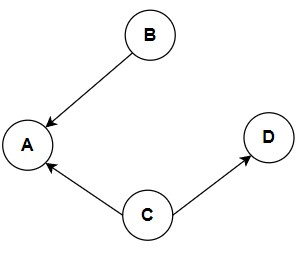
\includegraphics{graph_or.jpg}
        \caption{Ориентированный граф}
    \end{minipage}
    \hspace{3cm}
    \begin{minipage}[t]{4cm}
        \centering
        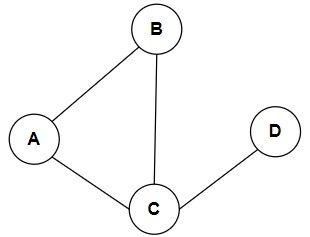
\includegraphics{graph_nor.jpg}
        \caption{Неориентированный граф}
    \end{minipage}
\end{figure*}

\textbf{Висячей вершиной} называется вершина, которая соединена только с одной соседней вершиной.

\textbf{Степенью вершины} называется количество ребер, соединенных с этой вершиной.
Если степень вершины равна 0, то такая вершина называется \textbf{изолированной}.
Степень вершины может быть \textbf{входящей} и \textbf{исходящей}. Входящая степень вершины $v$
это количество ребер вида $\langle i, v \rangle$, то есть количество ребер которые входят в $v$.
Исходящая степень вершины $v$ это количество ребер вида $\langle v, i \rangle$, то есть количество ребер
которые входят из $v$.

\begin{thm}
    В любом графе всегда найдутся хотя бы две вершины с одинаковой степенью.
\end{thm}

Дуга, у которой начало и конец совпадают, называется \textbf{петлей}.

Граф $\langle M', N'\rangle$ называется \textbf{простым путем}, если
\begin{enumerate}
    \item число его дуг $k$ на единицу меньше числа вершин
    \item можно так пронумеровать $M'$ числами от 0 до $k$ и $N'$ числами от 1 до $k$,
    что для любой дуги $u \in N'$
\end{enumerate}

Пусть $num$ - это получение номера дуги или вершины, а $beg(u)$ и $end(u)$ начало и конец дуги 
$u$ соответственно. Тогда для любой дуги $u$ в графе верно выражение:
\begin{equation}
    \label{simple_path}
    num(u) = num(end(u)) = num(beg(u)) + 1
\end{equation}
Различие между \textbf{путем} и \textbf{простым путем} заключается в том, что во втором случае
недопустимы повторы вершин и дуг в пути.
\begin{figure}[h]
    \centering 
    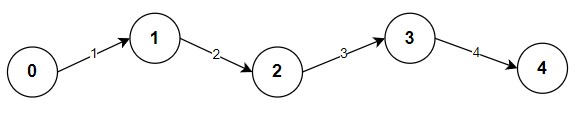
\includegraphics{simple_path.jpg}
    \caption{Простой путь}
\end{figure}

\begin{thm}
    Простым графом называется граф, который не имеет петель и не содержит более чем одно ребро между вершинами.
\end{thm}
Граф $\langle M', N'\rangle$ называется \textbf{цепью}, если:
\begin{enumerate}
    \item число его дуг $k$ на единицу меньше числа вершин
    \item можно так пронумеровать $M'$ числами от 0 до $k$ и $N'$ числами от 1 до $k$,
    что для любой дуги $u \in N'$
\end{enumerate}
То есть, он включает либо условие простого пути \ref{simple_path}, либо
\begin{equation}
    \label{chain}
    num(u) = num(end(u)) + 1 = num(beg(u))
\end{equation}
Дуги, для которых выполняется \ref{simple_path}, принято называть \textbf{положительно ориентированными},
а те, для которых выполняется \ref{chain} \textbf{отрицательно ориентированными}.

\begin{figure}[h]
    \centering 
    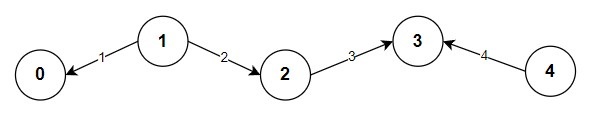
\includegraphics{chain.jpg}
    \caption{Цепь}
\end{figure}

Граф $\langle M', N'\rangle$ называется \textbf{контуром}, если
\begin{enumerate}
    \item число дуг $k$ равно числу вершин
    \item можно так пронумеровать $M'$ и $N'$ числами от 1 до k, что для любой
    дуги $u \in N'$
\end{enumerate}
\begin{equation}
    num(u) \stackrel{\text{mod k}}{=} num(end(u)) \stackrel{\text{mod k}}{=} num(beg(u)) + 1
\end{equation}
Иными словами, контур - это простой путь, где начало и конец совпадают.

\begin{figure}[h]
    \centering 
    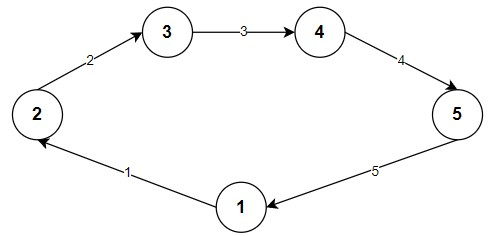
\includegraphics{loop.jpg}
    \caption{Контур}
\end{figure}

\vspace{3mm}

Граф $\langle M', N'\rangle$ называется \textbf{циклом}, если
\begin{enumerate}
    \item число дуг $k$ равно числу вершин
    \item можно так пронумеровать $M'$ и $N'$ числами от 1 до $k$, что для любой дуги $u \in N'$
\end{enumerate}
\begin{equation}
    num(u) \stackrel{\text{mod k}}{=} num(end(u)) \stackrel{\text{mod k}}{=} num(beg(u)) + 1
\end{equation}
либо
\begin{equation}
    num(u) \stackrel{\text{mod k}}{=} num(end(u)) + 1 \stackrel{\text{mod k}}{=} num(beg(u))
\end{equation}
Цикл - это цепь, в которой начало и конец совпадают.
\begin{figure}[h]
    \centering 
    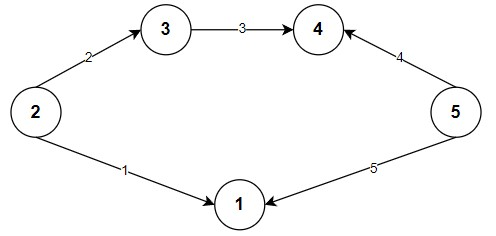
\includegraphics{cycle.jpg}
    \caption{Цикл}
\end{figure}

\section{Связность. Компоненты связности и сильной связности}
Граф $\langle M, N\rangle$ называется \textbf{связным}, если любые две различные его
вершины можно соединить цепью. Любой граф может быть однозначно разделен на максимальные
связные подграфы, которые называют его \textbf{компонентами связаности}.
c

Граф $\langle M, N\rangle$ называется \textbf{сильно связным}, если любые две различные
вершины A и B можно соединить путем с началом в A и концом в B. В любом графе можно однозначно
выделить максимальные сильно связные подграфы, которые называются его \textbf{компонентами сильной связности}.
\begin{thm}
    Граф компонент сильной связности не имеет контуров.
\end{thm}

\section{Матричные представления графов}
Прежде чем приступить к понятию "дерево" , изучим различные способы представления графов.
Наиболее известные формы это \textbf{матрица инцидентности} и \textbf{матрица смежности}.
Для начала рассмотрим более простой вариант - матрицу смевжности.

\vspace{3mm}

\textbf{Матрицей смежности} графа $\langle M, N\rangle$ называется такая квадратная матрица $M \times M$
(то есть индексами строк и столбцов являются вершины графа), 
в которой значением пересечения $i$-ой строки и $j$-го столбца является число дуг с началом в $i$ и концом $j$.

\begin{figure}[!h]
    \centering 
    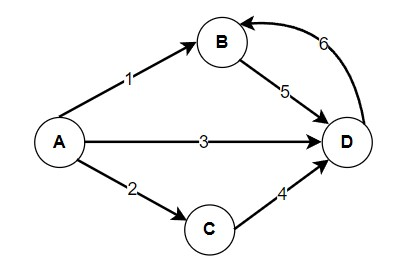
\includegraphics{graph_1.jpg}
    \caption{Граф}
    \label{graph_for_matrix}
\end{figure}

\begin{figure*}[!h]
    \centering
    \begin{minipage}[t]{4cm}
        \centering
        \begin{tabular}[c]{ | l | l | l | l | l | l | l | l |}
            \hline
              & 1  & 2  & 3  & 4  & 5  & 6  \\ \hline
            A & 1  & 1  & 1  & 0  & 0  & 0  \\ \hline
            B & -1 & 0  & 0  & 0  & 1  & -1 \\ \hline
            C & 0  & -1 & 0  & 1  & 0  & 0  \\ \hline
            D & 0  & 0  & -1 & -1 & -1 & 1  \\
            \hline
        \end{tabular}
    \end{minipage}
    \hspace{3cm}
    \begin{minipage}[t]{4cm}\
        \centering
        \begin{tabular}[c]{ | l | l | l | l | l |}
            \hline
              & A & B & C & D \\ \hline
            A & 0 & 1 & 1 & 1 \\ \hline
            B & 0 & 0 & 0 & 1 \\ \hline
            C & 0 & 0 & 0 & 1 \\ \hline
            D & 0 & 1 & 0 & 0 \\
            \hline
        \end{tabular}
    \end{minipage}
    \caption{Способы матричного представления графа \ref{graph_for_matrix}: матрица инцидентности
    и матрица смежности соответственно}
\end{figure*}

\hspace{3mm}

\textbf{Матрицей инцидентности} графа $\langle M, N\rangle$ называется такая матрица $M \times N$, 
где индексами строк являются вершины, а индексами столбцов дуги. Элемент на пересечении $i$-ой строки и $j$-ого
столбца равен 1, если является началом в вершине под $i$-ым индексом и принадлежит дуге под $j$-ым индексом. Если же данная
дуга имеет конец в этой вершине, то ставится -1.

\section{Деревья}
Чтобы ввести термин "дерево", нам нужно изучить следующую теорму:
\begin{thm}
    В связном графе $\langle M, N \rangle$ найдется частичный граф связный граф
    $\langle M, N' \rangle$, в котором количество вершин больше количества дуг на единицу. Пусть $|N'| = k$, 
    тогда если пронумеровать вершины из M числами от 0 до k, а дуги из N' числами от 1 до k
    таким образом, что для любой дуги $u \in N'$ выполняется соотношение
    \begin{equation}
        num(u) = max\{num(beg(u)), num(end(u))\}
    \end{equation}
\end{thm}
\begin{sle}
    Если $|N| < |M| - 1$, граф не может быть связан.
\end{sle}
\begin{sle}
    Если $|N| > |M| - 1$, граф содержит циклы.
\end{sle}

Связный граф без циклов, в котором число дуг на 1 меньше числа вершин, называется
\textbf{деревом}. Такие деревья могут не иметь корня, в отличие от тех деревьев,
которые мы обычно представляем. Если подобное дерево имеет корень, то оно называется 
\textbf{ориентированным деревом}.

\begin{thm}
    Для того, чтобы простой неориентированный граф с n вершинами был деревом необходимо 
    и достаточно, чтобы он был связен  и в нем было n-1 ребро.
\end{thm}
Дерево, являющееся частичным графом связного графа, называется его \textbf{остовным деревом} (spanning tree).

Теперь можно присутпить к изучению алгоритма нахождения остовного дерева методом вычеркивания.

\hspace{5mm}
\newpage

\section{Алгоритмы нахождения остовного дерева}
\textbf{Алгоритм ближайшего соседа}
\begin{enumerate}
    \item В весовой матрице выбираем произвольную вершину.
    \item Ищем в этой весовой вершине минимальную дугу в другую вершину.
    \item Ищем среди этих вершин снова минимальную дугу уже в новую вершину.
    \item Продолжаем до тех пор, пока не пометим все вершины.
\end{enumerate}
Приведем пример. Пусть есть следующая весовая матрица:

\begin{table}[h]
    \centering
    \begin{tabular}[c]{ | l | l | l | l | l | l | l | }
        \hline
          & A & B & C & D & E & F \\ \hline
        A & 0 & 0 & $\infty$ & 4 & 6 & $\infty$ \\ \hline
        B & 5 & 0 & $\infty$ & 7 & 5 & 4\\ \hline
        C & $\infty$ & $\infty$ & 0 & 5 & 6 & 4 \\ \hline
        D & 4 & 7 & 5 & 0 & 8 & 3\\ \hline
        E & 6 & 5 & 6 & 8 & 0 & $\infty$\\ \hline
        E & $\infty$ & 4 & 4 & 3 & $\infty$ & 0 \\
        \hline
    \end{tabular}
    \caption{Весовая матрица}
\end{table}

\begin{figure}[!h]
    \centering 
    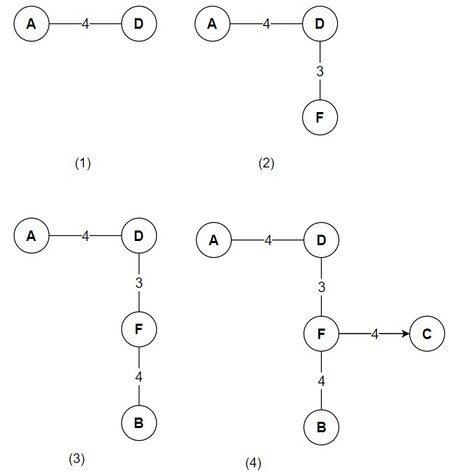
\includegraphics{kn.jpg}
    \caption{Алгоритм ближайшего соседа}
    \label{graph_kn}
\end{figure}

На рисунке \ref{graph_kn} изображен алгоритм построения остовного дерева для весовой матрицы выше. 
Пусть произвольная вершина будет A. Минимальное ребро идет в вершину D. 
Далее выбираем среди этих двух вершин минимальное ребро, и это D -> F. По такому же
алгоритму достраиваем остовное дерево.

\hspace{5mm}
\newpage
\textbf{Жадный алгоритм}

Этот алгоритм основан по большей части на том, что каждый раз мы выбираем минимальное ребро
на каждом этапе, а далее объединяем полученные ребра в остовное дерево. Для той же весовой матрицы покажем:
На рисунке \ref{greedy_alg} изображено построение остовного дерева с помощью жадного алгоритма.

\begin{figure}[!h]
    \centering 
    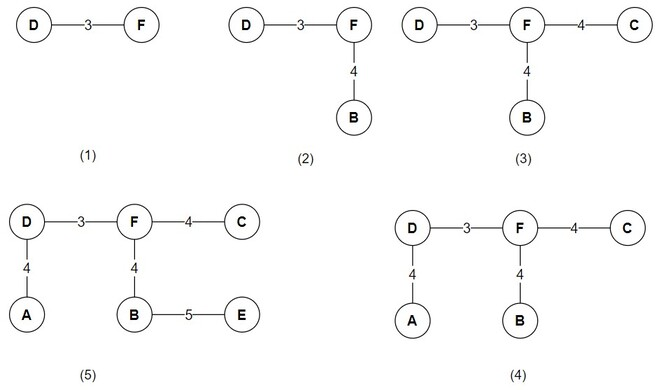
\includegraphics{greedy_alg.jpg}
    \caption{Жадный алгоритм}
    \label{greedy_alg}
\end{figure}

Самое минимальное ребро равно 3 с вершинами D и F. Далее мы имеем 3 равнозначеных ребра равных 4:
F и B, F и C, D и A. Строми последовательно их. Не хватает последнего ребра E. Можно заметить, что самое минимальное
ребро с этой вершиной из B. Остовное дерево построено.

\hspace{5mm}
\newpage
\textbf{Алгоритм вычеркивания}

\begin{enumerate}
    \item В матрице инцидентности $N \times N-1$ проверяем наличие нулевых строк. 
    Если есть, то имеем неостовное дерево.
    \item Если нет, то проверяем наличие строк с одной единицей
    и вычеркиваем строку и столбец, проходящие через эту единицу
    \item Повторяем пункт 1 и 2 до тех пор, пока не придем к выводу, что это неостовное дерево или
    если все столбцы вычеркнуты, то рассмотренные ребра образуют остовное дерево
\end{enumerate}

Рассмотрим пример. Имеем следующую матрицу инцидентности:
\begin{table}[!h]
    \centering
    \begin{tabular}[c]{ | l | l | l | l | l | l | l | l | l | l | }
        \hline
        1 & 2 & 3 & 4 & 5 & 6 & 7 & 8 & 9 & 10 \\ \hline
        1 & 0 & 0 & 1 & 0 & 1 & 0 & 0 & 0 & 0 \\ \hline
        0 & 1 & 0 & 0 & 0 & 0 & 0 & 0 & 1 & 1 \\ \hline
        1 & 1 & 1 & 0 & 0 & 0 & 0 & 0 & 0 & 0 \\ \hline
        0 & 0 & 0 & 0 & 0 & 1 & 1 & 1 & 0 & 0 \\ \hline
        0 & 0 & 1 & 0 & 0 & 1 & 1 & 0 & 0 & 0 \\ \hline
        0 & 0 & 0 & 1 & 1 & 0 & 0 & 0 & 0 & 0 \\ 
        \hline
    \end{tabular}
    \caption{Матрица инцидентности}
\end{table}
\newpage
Теперь проверим, являются ли ребра 1, 2, 5, 7 и 8 остовным деревом:
\begin{figure}[!h]
    \centering 
    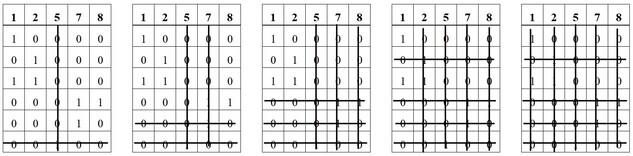
\includegraphics{matrix1.jpg}
    \caption{Алгоритм вычеркивания}
\end{figure}

Так как в процессе у нас не возникло нулевых строк и в итоге все строки и столбцы 
были зачеркнуты, данные ребра образуют остовное дерево.
Например, ребра 1, 2, 4, 5 и 8 не будут образовывать остовное дерево, так как 5
строчка будет состоять только из нулей.

\section{Задача о кратчайшем пути}
Для того чтобы найти кратчайший путь от одной вершины до других, используется алгоритм Дейкстры.
Алгоритм работает только для графов без рёбер отрицательного веса.

Алгоритм заключается в том, что каждой вершине соотвествует минимальное известное расстояние от
этой вершины до \textbf{a}. Метка вершины \textbf{a}, от которой ищутся кратчайшие расстояния до других, изначально равна 0, метки
остальных вершин равны бесконечности. Алгоритм работает пошагово - на каждом шаге он посещает одну вершину
и пытается уменьшать метки: из еще непосещенных вершин выбирается та, которая имеет
минимальную метку. Для каждого непосещенного соседа вершины, рассмотрим новую длину пути,
равную сумме значений текущей метки и длины ребра, соединяющего ее с этим соседом.
Если все вершины посещены, то работа алгоритма прекращается. Рассмотрим теперь пример:

\hspace{3mm}

Пусть требуется найти кратчайшие расстояния от 1-й вершины до всех остальных. 

\begin{figure}[!h]
    \centering
    \begin{tabular}{cc}
        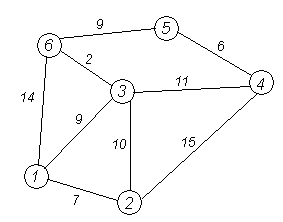
\includegraphics[scale=0.6]{dijkstra_1.png} & 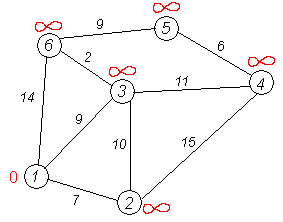
\includegraphics[scale=0.6]{dijkstra_2.png}
    \end{tabular}
\end{figure}

Кружками обозначены вершины, линиями — пути между ними (рёбра графа).
В кружках обозначены номера вершин, над рёбрами обозначен их вес — длина пути.
Рядом с каждой вершиной красным обозначена метка — длина кратчайшего пути в эту вершину из вершины 1. 

Минимальную метку имеет вершина 1. Её соседями являются вершины 2, 3 и 6.

Первый по очереди сосед вершины 1 — вершина 2, потому что длина пути до неё минимальна.
Длина пути в неё через вершину 1 равна сумме значения метки вершины 1 и длины ребра, идущего из 1-й в 2-ю, то есть 0 + 7 = 7.
Это меньше текущей метки вершины 2, бесконечности, поэтому новая метка 2-й вершины равна 7.
Аналогичную операцию проделываем с двумя другими соседями 1-й вершины — 3-й и 6-й.

\begin{figure}[!h]
    \centering 
    \begin{tabular}{cc}
        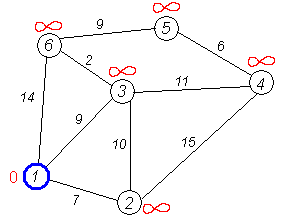
\includegraphics[scale=0.6]{dijkstra_3.png} & 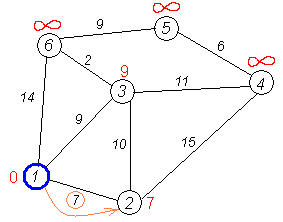
\includegraphics[scale=0.6]{dijkstra_4.png} \\
        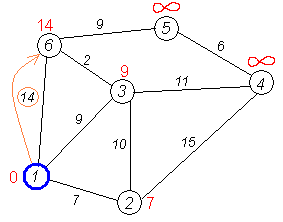
\includegraphics[scale=0.6]{dijkstra_5.png} & 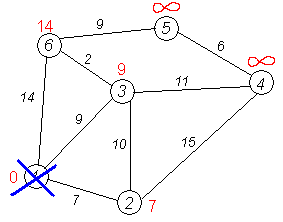
\includegraphics[scale=0.6]{dijkstra_6.png}
    \end{tabular}
\end{figure}

Все соседи вершины 1 проверены.
Текущее минимальное расстояние до вершины 1 считается окончательным и пересмотру не подлежит.
Вычеркнем её из графа, чтобы отметить, что эта вершина посещена. 

Снова находим «ближайшую» из непосещённых вершин. Это вершина 2 с меткой 7. 

\begin{figure}[!h]
    \centering 
    \begin{tabular}{cc}
        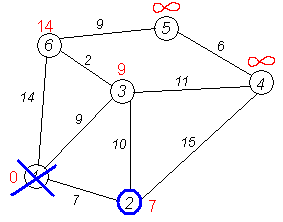
\includegraphics[scale=0.6]{dijkstra_7.png} & 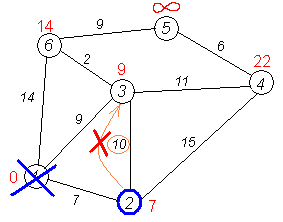
\includegraphics[scale=0.6]{dijkstra_8.png} \\
        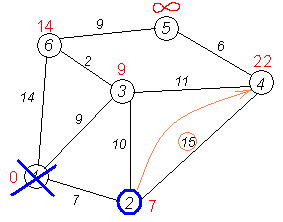
\includegraphics[scale=0.6]{dijkstra_9.png} & 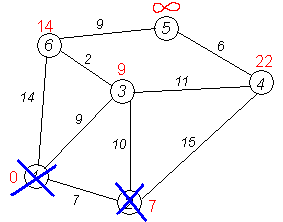
\includegraphics[scale=0.6]{dijkstra_10.png}
    \end{tabular}
\end{figure}

Снова пытаемся уменьшить метки соседей выбранной вершины, пытаясь пройти в них через 2-ю вершину. Соседями вершины 2 являются вершины 1, 3 и 4.
Первый (по порядку) сосед вершины 2 — вершина 1. Но она уже посещена, поэтому с 1-й вершиной ничего не делаем.
Следующий сосед — вершина 3, так как имеет минимальную метку.
Если идти в неё через 2, то длина такого пути будет равна 17 (7 + 10 = 17). Но текущая метка третьей вершины равна 9, а это меньше 17, поэтому метка не меняется. 
Ещё один сосед вершины 2 — вершина 4.
Если идти в неё через 2-ю, то длина такого пути будет равна сумме кратчайшего расстояния до 2-й вершины и расстояния между вершинами 2 и 4, то есть 22 (7 + 15 = 22).
Поскольку 22 < $\infty$ , устанавливаем метку вершины 4 равной 22.
Все соседи вершины 2 просмотрены, замораживаем расстояние до неё и помечаем её как посещённую. 

Проводим аналогичные шаги с другими вершинами и получаем в результате:

\begin{figure}[!h]
    \centering 
    \begin{tabular}{cc}
        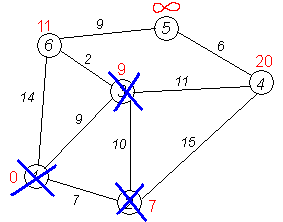
\includegraphics[scale=0.5]{dijkstra_11.png} & 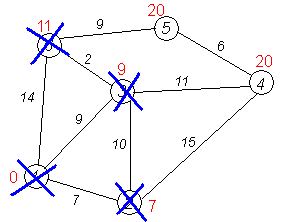
\includegraphics[scale=0.5]{dijkstra_12.png} \\
        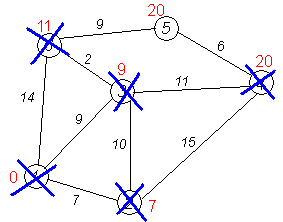
\includegraphics[scale=0.5]{dijkstra_13.png} & 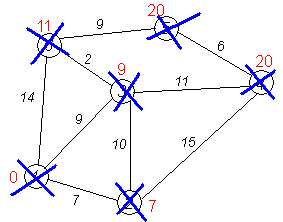
\includegraphics[scale=0.5]{dijkstra_14.png}
    \end{tabular}
\end{figure}

Алгоритм заканчивает работу, когда все вершины посещены.
Результат работы алгоритма виден на последнем рисунке: кратчайший путь от вершины 1 до 2-й составляет 7, до 3-й — 9, до 4-й — 20, до 5-й — 20, до 6-й — 11.
Если в какой-то момент все непосещённые вершины помечены бесконечностью, то это значит, что до этих вершин нельзя добраться (то есть граф несвязный). Тогда алгоритм может быть завершён досрочно. 


\chapter*{Литература}   
\begin{enumerate}
    \item Дискретный анализ. Романовский И.В.
    \item Дискретная математика и комбинаторика. Джеймс А. Андерсон
    \item Дискретная математика. Часть 1: Начальные понятия теории множеств и отношений,
    математическая логика. Некрасова М.Г.
\end{enumerate}

\shortlorem
\end{document}